\begin{problem}{자연공원}
	{}{}
	{2초}{256MB}{}
	
	JOI 섬은 섬 전체가 자연공원으로 지정된 관광지이다.
	
	JOI 섬에는 $N$ 개의 광장과 몇 개의 도로가 있다. 광장에는 0번부터 $N-1$번까지 번호가 붙어있다. 도로는 섬 내에 서로 다른 2개의 광장을 잇고, 양방향으로 이동할 수 있다. 어떤 광장에 대해서도 이 광장에 직접 연결된 도로는 최대 7개이다. 서로 다른 두 광장에 대해서 두 광장을 잇는 도로는 최대 한 개 존재한다. 몇 개의 도로를 거치면 한 광장에서부터 다른 광장으로 갈 수 있다.
	
	당신과 당신의 친구 IOI양은 JOI 섬을 탐험할 것이다. 효율적인 탐사를 위해 JOI 섬의 구조를 파악할 필요가 있다. 섬에는 위험한 야생동물이 많아 위험하므로 운동신경이 좋은 IOI양이 도시를 탐색하고 IOI양의 보고를 받아 당신이 섬의 구조를 파악하게 되었다.
	
	당신은 IOI양에게 두 광장의 번호 $A$, $B$와 경유 가능한 광장을 몇 개 지정하여 광장 $A$부터 광장 $B$까지 지정된 광장만 경유하여 이동하는 것이 가능하냐는 질문을 한다. IOI양은 질문의 내용을 따라 섬을 탐색하여 결과를 보고한다.
	
	조사에 긴 시간이 사용되면 위험하기 때문에 질문 횟수는 45 000번 이내여야 한다.
	
	\Specification
	
	당신은 섬의 구조를 파악하는 방법이 구현된 하나의 파일을 작성해야 한다. 이 파일은 \texttt{park.h}를 include해야 한다.
	
	이 파일에는, 다음 함수가 작성되어 있어야 한다.
	
	\begin{itemize}
		\item \texttt{void Detect(int T, int N)}
		
		이 함수는 한 번만 불린다.
		\begin{itemize}
			\item 인자 \texttt{T}는 서브태스크의 번호, \texttt{N}은 광장의 개수를 의미한다.
		\end{itemize}
		
		프로그램 안에서 다음의 함수를 호출하여, JOI 섬의 구조를 출력해야 한다.
		\begin{itemize}
			\item \texttt{void Answer(int A, int B)}
			
			이 함수의 호출 횟수는 JOI 섬의 도로의 개수와 같아야 한다.
			
			\begin{itemize}
				\item 인자 \texttt{A}, \texttt{B}는 \texttt{A}번 광장과 \texttt{B}번 광장 사이에 도로가 있다는 것을 의미한다.
			\end{itemize}
		
			함수 인자는 다음과 같은 조건을 만족해야 한다:
		
			\begin{itemize}
				\item \texttt{A}, \texttt{B}는 $0 \le $\texttt{A}$ < $\texttt{B}$ \le N-1$을 만족해야 한다. 이 조건을 만족하지 않으면 \textbf{오답 [1]}이 된다.
				\item 함수가 인자 (\texttt{A}, \texttt{B})로 호출되었으면 \texttt{A}번 광장과 \texttt{B}번 광장을 잇는 도로가 있어야 한다. 이 조건을 만족하지 않으면 \textbf{오답 [2]}이 된다.
				\item 이 함수는 같은 인자 (\texttt{A}, \texttt{B})로 두 번 이상 호출되면 안 된다. 이 조건을 만족하지 않으면 \textbf{오답 [3]}이 된다.
			\end{itemize}
		\end{itemize}
	
		또한, 당신의 프로그램은 다음 함수를 호출 할 수 있다.
		
		\item \texttt{int Ask(int A, int B, int Place[])}
		
		이 함수는 IOI양에게 질문을 하는 데에 쓰인다.
		\begin{itemize}
			\item \texttt{Place}는 경유할 수 있는 광장들의 배열을 가리키는 포인터이다. 각 $i$ ($0 \le i \le N-1$)에 대해, \texttt{Place[}$i$\texttt{]}$=1$이면, $i$번 광장을 경유할 수 있다는 의미이고, \texttt{Place[}$i$\texttt{]}$=0$이면, $i$번 광장을 경유할 수 없다는 의미이다.
			\item 이 함수의 반환 값은 \texttt{A}번 광장에서 \texttt{B}번 광장으로 배열 \texttt{Place[]}에 주어진 광장만으로 이동할 수 있으면 1이고, 아니면 0이다.
		\end{itemize}
	
	
		함수 인자는 다음과 같은 조건을 만족해야 한다:
		
		\begin{itemize}
			\item $0 \le $\texttt{A}$ < $\texttt{B}$ \le N-1$
			\item $0 \le$\texttt{Place[}$i$\texttt{]}$\le 1$  ($0 \le i \le N-1$)
			\item \texttt{Place[A]}$=1$
			\item \texttt{Place[B]}$=1$
		\end{itemize}
	
		위 조건들을 만족하지 않으면 \textbf{오답 [4]}이 된다. 하지만 배열 \texttt{Place[]}의 길이가 $N$이 아니면 이 함수의 동작은 보장되지 않는다.
		
		함수 \texttt{Ask}는 45 000번 초과로 호출되어서는 안 된다. 만약 초과하는 경우, \textbf{오답 [5]}이 된다.
		
	\end{itemize}

	함수가 종료되었을 때, \texttt{Answer}의 호출로 출력되지 않은 도로가 있는 경우에는 \textbf{오답 [6]}이 된다.
	
	당신의 프로그램은 내부에서 사용할 목적으로 함수나 전역변수를 사용할 수 있다. 당신의 프로그램은 표준 입출력을 사용해서는 안 된다. 당신의 프로그램은 어떠한 방법으로도 다른 파일에 접근해서는 안 된다. 
	
	당신은 대회 홈페이지의 아카이브에서 프로그램을 테스트하기 위한 목적의 샘플 그레이더를 받을 수 있다. 아카이브는 당신의 프로그램의 예제 소스 또한 첨부되어 있다.
	샘플그레이더는 파일 \texttt{grader.c} 혹은 \texttt{grader.cpp}이다. 당신의 프로그램이 \texttt{park.c} 혹은, \texttt{park.cpp} 인 경우 다음 커맨드로 컴파일할 수 있다.
	
	\begin{itemize}
		\item C
		\texttt{g++ -std=c11 -O2 -o grader grader.c park.c -lm}
		\item C++
		\texttt{g++ -std=c++14 -O2 -o grader grader.cpp park.cpp}
	\end{itemize}
	
	컴파일이 성공적이면, 파일 \texttt{grader}가 생성된다.
	
	실제 그레이더와 샘플 그레이더는 다름에 주의하여라. 샘플 그레이더는 하나의 프로세스에서 실행되며, 입력을 표준 입력으로부터 받고, 출력을 표준 출력에 출력한다.
	
	\InputFile
	
	샘플 그레이더는 다음 형식으로 표준 입력으로부터 데이터를 입력받는다.
	
	\begin{itemize}
		\item 첫 번째 줄에 서브태스크의 번호 $T$가 주어진다.
		\item 두 번째 줄에 광장의 개수 $N$이 주어진다.
		\item 세 번째 줄에 도로의 개수 $M$이 주어진다.
		\item 다음 $M$ 개의 줄의 $i$ 번째 ($1 \le i \le M$) 줄에는 공백으로 구분된 두 정수 $A_i$, $B_i$가 주어진다. 이는 $A_i$번 광장과 $B_i$번 광장을 잇는 도로가 있어서 양방향으로 오갈 수 있다는 의미이다.
	\end{itemize}
	
	
	\OutputFile
	
	프로그램이 정상적으로 종료되었다면, 샘플 그레이더는 다음과 같은 정보를 표준 출력에 출력한다. (따옴표는 출력하지 않는다.)
	
	\begin{itemize}
		\item 프로그램이 정답으로 판단된 경우에는,  ``\texttt{Accepted.}"를 출력한다.
		\item 오답으로 판단된 경우, 오답의 종류를 ``\texttt{Wrong Answer [1]}"과 같은 형식으로 출력하고 프로그램이 종료된다.
	\end{itemize}
	
	프로그램이 다양한 오답의 종류에 속해 있으면 샘플 그레이더는 그중 하나만 출력할 것이다.
	
	\Constraints
	
	$T$, $N$, $M$의 의미에 대해서는 입력 형식을 참고하여라.
	
	\begin{itemize}
		\item $1 \le T \le 5$.
		\item $2 \le N \le 1\ 400$.
		\item $1 \le M \le 1\ 500$.
		\item 어떤 광장에 대해서도 이 광장에 직접 연결된 도로는 최대 7개이다.
		\item 몇 개의 도로를 거치면 한 광장에서부터 다른 광장으로 갈 수 있다.
		\item 서로 다른 두 광장에 대해서 두 광장을 잇는 도로는 최대 한 개 존재한다.
	\end{itemize}
	
	

	\SubtaskWithCost{1}{10}
	\begin{itemize}
		\item $T = 1$.
		\item $N \le 250$.
	\end{itemize}
	
	\SubtaskWithCost{2}{10}
	\begin{itemize}
		\item $T = 2$.
		\item $M = N-1$.
		\item 0번과 $N-1$번 광장에 대해 다른 광장으로 가는 도로가 정확히 한 개 존재한다. 다른 모든 장소에 대해서는 다른 광장으로 가는 도로가 정확히 두 개 존재한다.
	\end{itemize}
	
	\SubtaskWithCost{3}{27}
	\begin{itemize}
		\item $T = 3$.
		\item $M = N-1$.
		\item 모든 $i$ ($0 \le i \le N-1$)에 대해, 0번 광장으로부터 $i$번 광장으로까지 최대 8개의 다른 광장을 거치면 오갈 수 있다.
	\end{itemize}
	
	
	\SubtaskWithCost{4}{30}
	\begin{itemize}
		\item $T = 4$.
		\item $M = N-1$.
	\end{itemize}
	
	
	\SubtaskWithCost{5}{23}
	\begin{itemize}
		\item $T = 5$.
	\end{itemize}
	
	\Examples
	
	예제 입력과 이에 해당하는 함수 호출을 보여준다. 
	
	\begin{tabular}{|l|l|l|}
		\hline
		\multirow{2}{*}{예제 입력}                                                                                        & \multicolumn{2}{l|}{예제 함수 호출}    \\ \cline{2-3} 
		& 호출                         & 반환값 \\ \hline
		\multirow{10}{*}{\begin{tabular}[c]{@{}l@{}}\texttt{1}\\ \texttt{6}\\ \texttt{7}\\ \texttt{0 1}\\ \texttt{0 3}\\ \texttt{1 2}\\ \texttt{1 4}\\ \texttt{2 4}\\ \texttt{2 5}\\ \texttt{3 4}\end{tabular}} & \texttt{Ask(3, 5, \{0,0,1,1,1,1\})} & 1   \\ \cline{2-3} 
		& \texttt{Answer(2, 4)}               &     \\ \cline{2-3} 
		& \texttt{Answer(3, 5)}               &     \\ \cline{2-3} 
		& \texttt{Answer(3, 4)}               &     \\ \cline{2-3} 
		& \texttt{Ask(0, 4, \{1,0,1,0,1,0\})} & 0   \\ \cline{2-3} 
		& \texttt{Answer(0, 1)}               &     \\ \cline{2-3} 
		& \texttt{Answer(0, 3)}               &     \\ \cline{2-3} 
		& \texttt{Answer(1, 4)}               &     \\ \cline{2-3} 
		& \texttt{Answer(1, 2)}               &     \\ \cline{2-3} 
		&                            &     \\ \hline
	\end{tabular}

	이 함수 호출이 꼭 의미가 있는 것은 아니다.
	
	이 예제에서, 함수 \texttt{Detect}는 인자 \texttt{T}$=1$, \texttt{N}$=6$으로 호출되었다.
	
	이 예제에서, JOI 섬의 구조는 다음과 같다.
	
	
	\begin{center}
	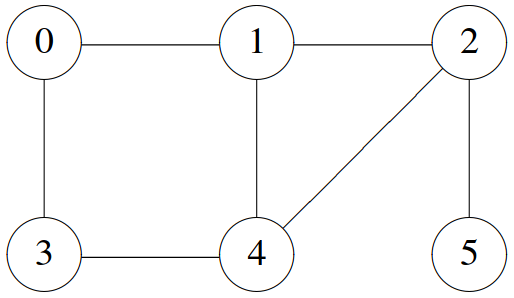
\includegraphics[width=0.3\linewidth]{pic1.png}
	
	JOI 섬의 구조
	\end{center}
	원과 숫자는 광장과 그 번호를 의미한다. 선분은 도로를 의미한다.
	
	\begin{itemize}
		\item 첫 번째 \texttt{Ask} 함수 호출은 3번 광장부터 5번 광장까지 2, 3, 4, 5번 광장만 경유하여 갈 수 있는지를 물어보았다. 가능하므로, 함수 \texttt{Ask}는 1을 반환한다.
		\item 두 번째 \texttt{Ask} 함수 호출은 0번 광장부터 4번 광장까지 0, 2, 4번 광장만 경유하여 갈 수 있는지를 물어보았다. 불가능하므로, 함수 \texttt{Ask}는 0을 반환한다.
	\end{itemize}
	
\end{problem}

